\chapter{SAFE Wiki}

SAFE Wiki is an application that allows users to both upload and browse content that can be stored in a ZIM file. The ZIM file format allows you to easily store content from the web, one of its uses is in the distribution of Wikimedia based content.

\section{Kiwix}

Kiwix first launched in 2007 as a way to browse the internet ``offline''. It achieves this through the use of ZIM files which are suitable for storing most HTML based content. One of the primary goals of Kiwix is to allow users to browse Wikipedia and other projects from the Wikimedia foundation without an internet connection. Whether this be in the middle of the ocean, Africa or even inside North Korea. Since the initial launch, different versions of the software have been released. Versions support many different platforms including: iOS, Android, Windows Phone, FireFoxOS, macOS, Windows and Linux. A user opens the app and then through a file explorer (or other means) selects the target ZIM file. Kiwix then presents the user with an almost ``web browser like'' experience. With resources like Wikipedia it looks uncannily like the real thing. Users have the ability to follow hyperlinks around the website (ZIM file) and search for pages. The London page of Wikivoyage can be seen in \textit{Figure \ref{fig:kiwix-firefox}}. With such a fantastic history behind the project, Kiwix was seen as the natural foundation to build SAFE Wiki upon. Kiwix is inherently a \textit{Fat Client} style of application as all processing is done on the client. Hence building upon an already \textit{Fat Client} application made perfect sense considering the points made in Chapter \ref{ch:thesafenetwork}. SAFE Wiki would do all the processing/reading of the file locally and use the SAFE Network as the storage medium for ZIM files.

\subsection{Kiwix JS}

Kiwix JS is a JavaScript variant of Kiwix, originally part of the Evopedia project it presents Kiwix in the form of a browser extension. This extension has support for many different environments (FireFox, Chrome, Edge, etc) due to the portable nature of Javascript.

As the SAFE Network is still very much in its infancy the developer API's reflect this. At the time of writing the only API's that are ready for use are the \textit{Node.js API} and what they call the \textit{Web API}. The \textit{Web API} can be used to build websites to interact with the SAFE Network whereas the \textit{Node.js API} facilitates the development of desktop applications. Both of these require the usage of JavaScript, hence forking Kiwix JS to build SAFE Wiki made logical sense.

\begin{figure}
	\begin{center}
			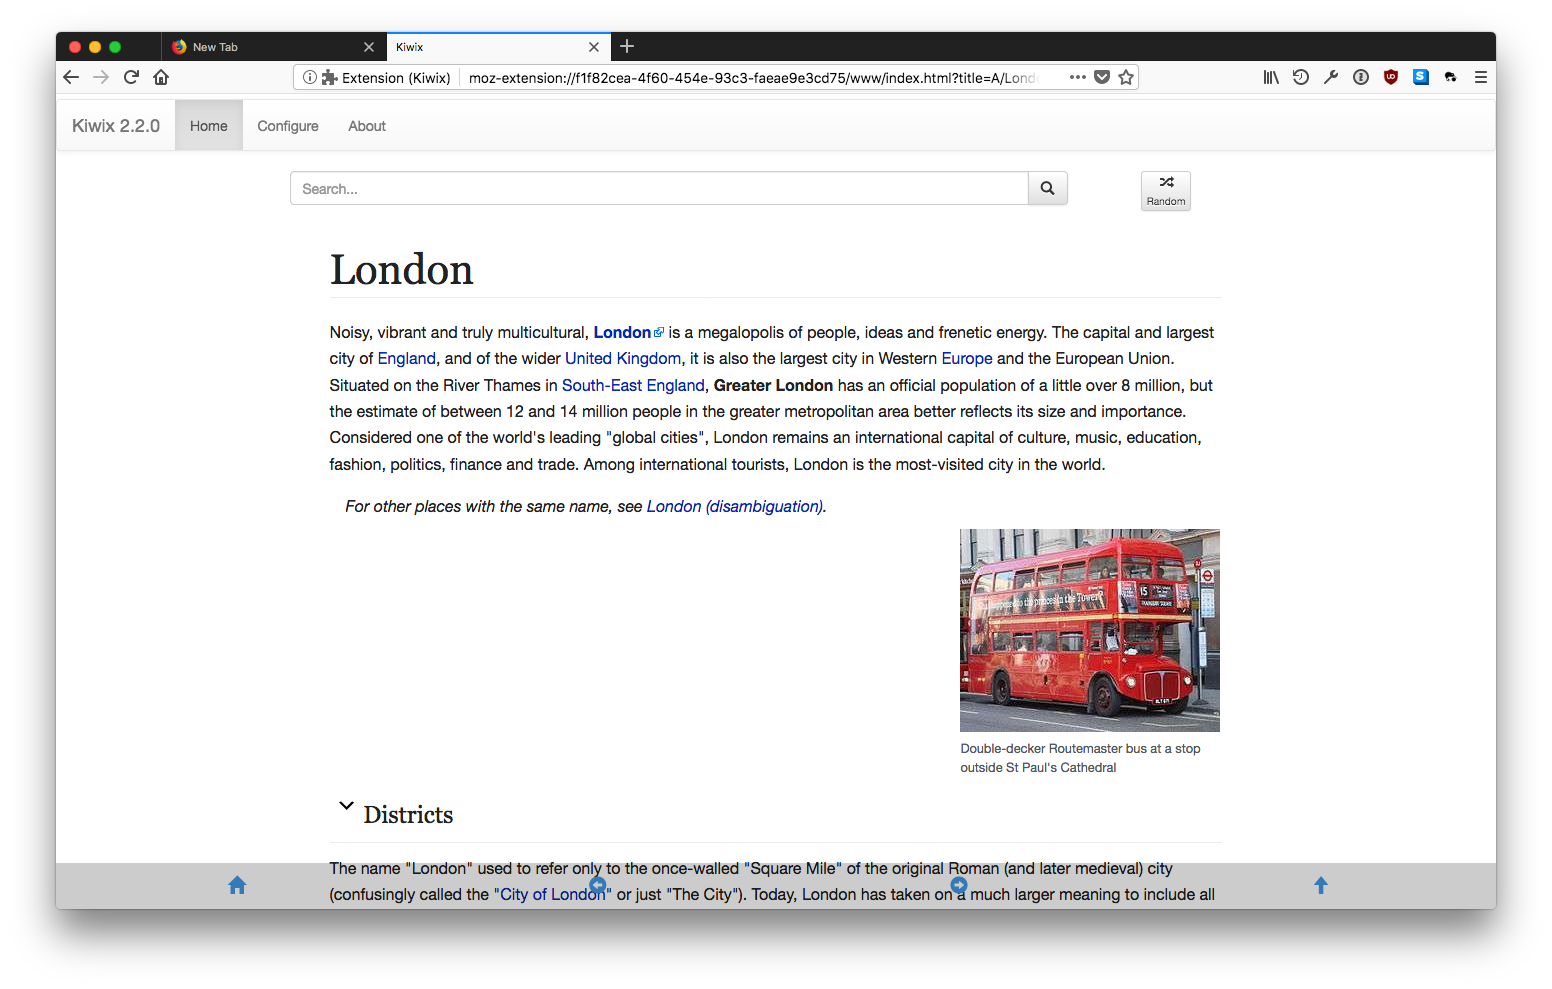
\includegraphics[width=\textwidth]{images/kiwix-js-extension}
		\caption{Kiwix-JS running in FireFox}
		\label{fig:kiwix-firefox}
	\end{center}
\end{figure}

Kiwix JS as it stands has support for Wikimedia and StackOverflow ZIM files (although others may work, just not supported). This meant that that through SAFE Wiki it would be possible to not only browse Wikimedia content but also content coming from StackOverflow. The content that users would be able to browse would be static, ZIM files are not mutable. The ZIM files being static does however bring its own benefits.

\section{Static versus Dynamic Content}

When the idea to ``build a Wikipedia on the SAFE Network'' was born, we were very well aware of the fact that it might just forever be a ``tech demo''. Getting enough users to start contributing content, and building an environment where strict moderation could occur, would have been a fools-errand given the time permissible for this project. It just wouldn't have been able to build a full Wiki system on the network and do it justice.

It is with that realisation that lead to the discovery of Kiwix. Instead of trying to build a Wiki system on the SAFE Network and trying to bring users across, it would be possible to bring Wikipedia (and other sites) to the SAFE Network. The content would not be dynamic in anyway (meaning the content couldn't be mutated) but it would be there for consumption. An important thing about this approach is that by the end of the year there would be a way to store a browsable copy of Wikipedia on the SAFE Network. In its entirety. Not just a simple throwaway tech demo but a tool that people might actually be able to use.

Websites like Wikipedia only work because of their user base. When a user edits an article this change is logged and anyone can review the changes made. As there are thousands of users anything that is grievously wrong is likely to be flagged and addressed quickly. If someone is acting as a \textit{bad-party} and editing pages wrongfully they can be blocked based on IP address. A simple example is a school, It does not need explaining that school children can be known for being rather silly sometimes. This behaviour can result in the vandalism of some Wikipedia pages. In such cases Wikipedia has the moderation tools to block the IP address(s) that belongs to a school (from making edits) and prevent any further vandalism. On the SAFE Network, this approach is impossible. A user could simply create another account and vandalise an open wiki all they want. It is for reasons such as this that building a dynamic wiki (with adequate moderation techniques/tools) would have been very difficult. A static mirror of Wikipedia was however very achievable.

A static version of Wikipedia might at first seam quite rigid, but in the context of the SAFE Network it makes sense. As the network has a concept of \textit{ownership of data}, a ZIM file can be directly tied to the original uploader. The ZIM file ``belongs'' to the account who uploaded the file and created the \textit{Data Map}. An organisation like Wikimedia, or a trusted third-party, can then upload ZIM files to the network with the assurance that users will know it came from them. It will then exist on the network as an un-censorable mirror (or archive) of whatever source the ZIM file came from. Everyone that has access to the SAFE Network can browse it, the only person that is allowed to ``remove'' access to the \textit{Data Map} is the original uploader. As long as a user trusts the source of the ZIM file and the address given to them for that file, they can \textit{trust} that the information contained within it came from them.

\section{Electron}

Electron allows you to ``Build cross platform desktop apps with JavaScript, HTML, and CSS''. Being able to produce an application that was cross platform was very important. The SAFE Network is not platform specific so SAFE Wiki should not have been either. As Kiwix JS is built upon web-technologies, Electron seamed like the obvious answer as to how to pull Kiwix JS outside of the web browser. Electron combines \textit{Node.js} and \textit{Chromium} into a single environment that can be deployed to the three main platforms: Windows, Linux and macOS. As there exists a \textit{Node.js API} for the SAFE Network it meant that a single application could be built. An application that could handle both the publishing of ZIM files and facilitate the browsing of them. The decision not to use the \textit{Web API} was because of file uploading. To facilitate the upload of large files, (The ZIM for Wikipedia with images is \textgreater 70GB) it really needed to build a desktop application.

\begin{figure}[h]
	\begin{center}
		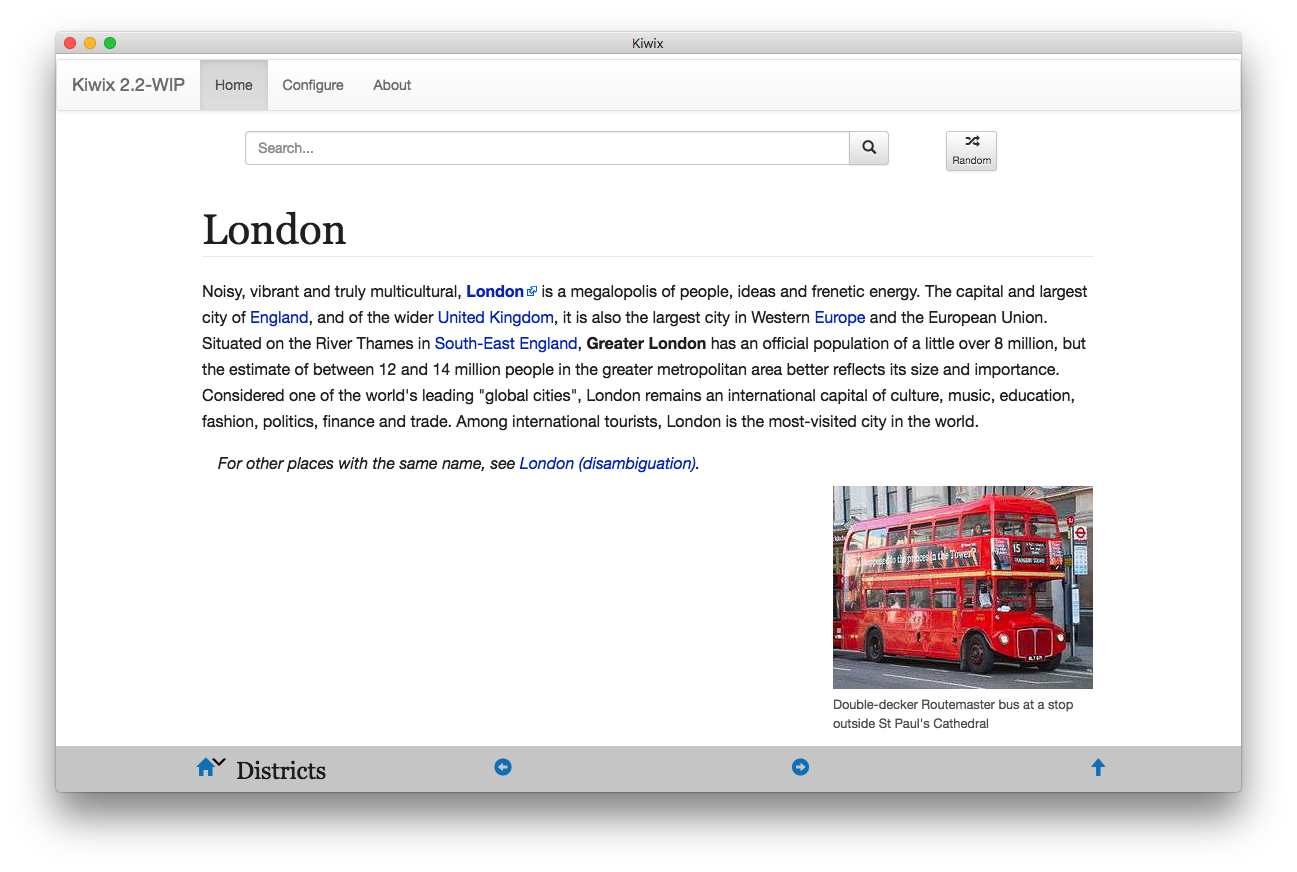
\includegraphics[width=\textwidth]{images/kiwix-js-electron}
		\caption{Kiwix JS as an Electron App}
		\label{fig:kiwix-js-electron}
	\end{center}
\end{figure}

Electron and \textit{Node.js} were unfamiliar technologies when development started. Making Kiwix JS run as an Electron application was hence quite a challenge. After a few months of work Kiwix JS was running in a desktop application. Indeed the creators of Kiwix had a similar idea of bundling Kiwix JS into an Electron application some time ago. They were pleased when contacted about the early success of this project. What was now SAFE Wiki (which can be seen in Figure \ref{fig:kiwix-js-electron}) could browse ZIM files from local storage and maintained all the functionality of Kiwix JS.

\section{Developing with the SAFE Network}

The SAFE Network was exceedingly difficult to work with, this was down to the lack of documentation and developer resources. Being only at `Alpha 2' they still have a long way to go before a true `1.0' release of the product. It is down to this development roadmap that indicates they are holding off on writing proper documentation until closer to the full release. The only saving grace in this matter was the Developer Forum. The Developer Forum is a very lively place with constant chatter, everyone pitches in and shares ideas. All the information needed to build SAFE Wiki was contained within the forums. This was not an optimal way to find the knowledge needed, it made work very slow and much harder than it needed to be. The lack of documentation and \textit{cannon} knowledge on certain topics resulted in the creation of several forum posts to help support this project. Users could not have been more helpful and most queries posted were resolved within a matter of days.

Development first starts with how to orchestrate the connection to the network. During development SAFE Browser was used, a fork of the Beaker Browser project. SAFE Browser takes the form of a web browser. Through it you can authenticate yourself with the network and browse any websites that are hosted on the SAFE Network, just like you can with a ``traditional'' web browser. If you build a standalone application, like SAFE Wiki, you can use IPC to communicate with SAFE Browser to gain authentication with the network. Once you have authentication you can communicate with the network directly meaning you don't need to use SAFE Browser as a middle man. Currently Maidsafe are working on the successor to SAFE Browser called Peruse. 

\begin{figure}[h]
	\begin{center}
		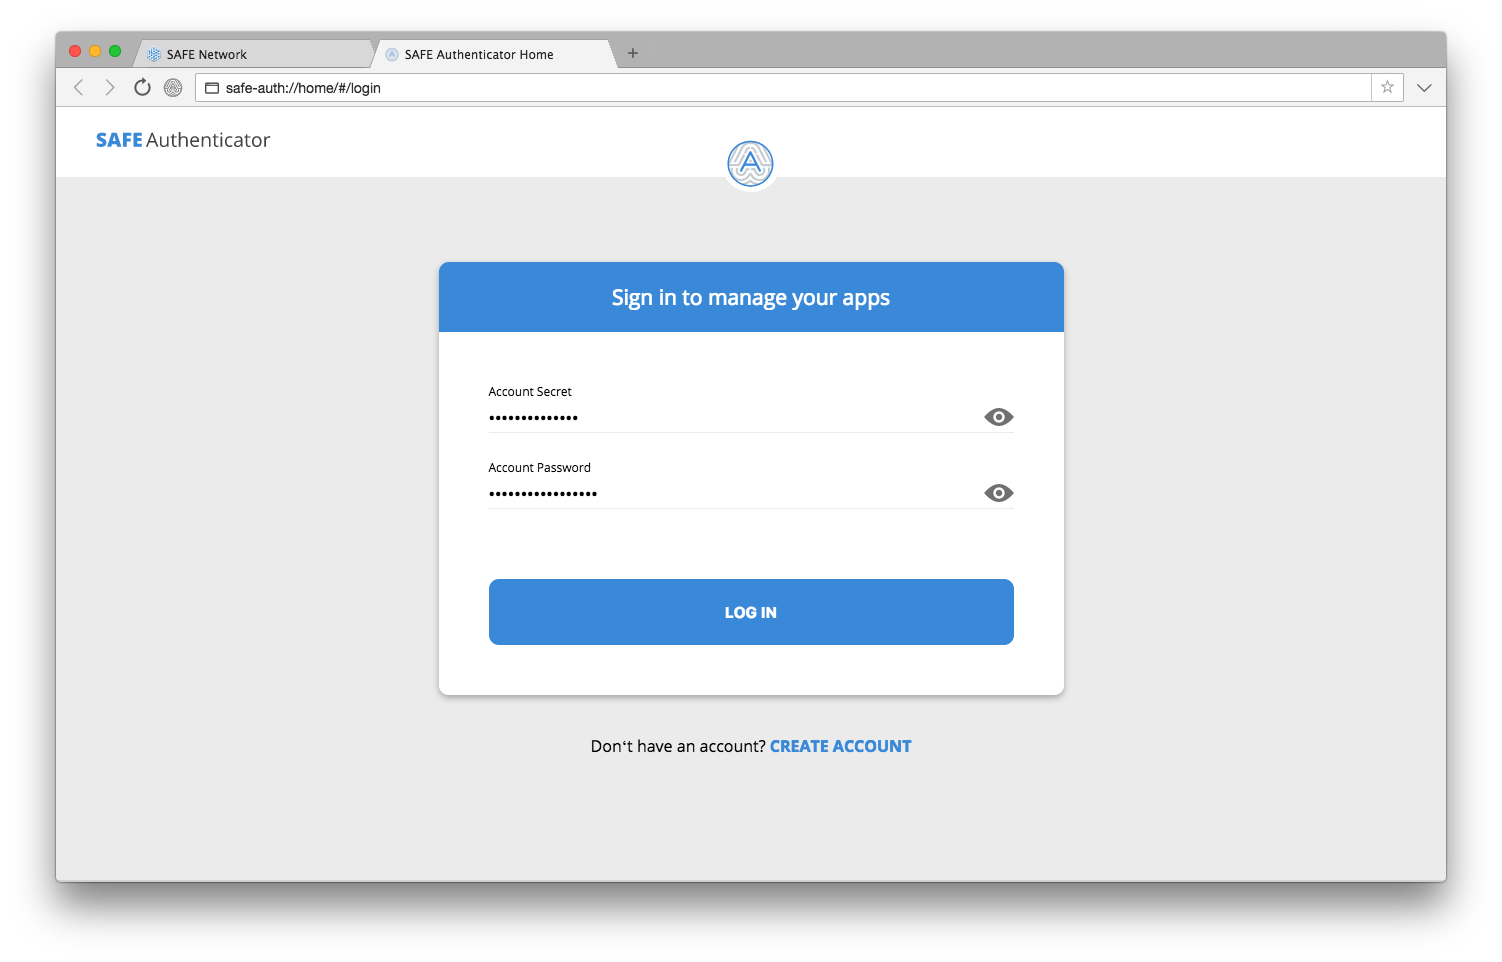
\includegraphics[width=\textwidth]{images/safe-browser-login}
		\caption{Login screen of the SAFE Browser}
		\label{fig:safe-browser-login}
	\end{center}
\end{figure}

To develop with the network you need to have some way of running your own ``development'' SAFE Network. There are currently three ways of achieving this.
\begin{itemize}
	\item Alpha 2 Network: This public network is hosted and ran by Maidsafe themselves. It is the ``official'' network for early adopters to host websites and run applications against. As it is a public network, it is not optimal for developmental work.
	\item Mock Routing: Mock routing is a technique that is baked into the SAFE Browser and Peruse. What it does is spoof the underlying network to the client through the use of a local database. This means that the client thinks it is talking to a real network while in actuality it is talking to a database. This is a very reliable way of developing locally, although it doesn't give you the full experience of how your application/web-site would work with a ``real'' SAFE Network. What this method does offer is simplicity. As it is built into the SAFE Browser you only need to download that single application. You just start SAFE Browser (with mock-routing support turned on) and you just work with it as you please.
	\item Local Network: Running a local SAFE Network is my preferred choice. Sadly it was very long into development before it was discovered just how easy it was to run a ``real'' SAFE Network locally. The process isn't as simple as downloading the binaries and clicking run, but it is not difficult. One has to download and compile the ``safe\_vault'' from Maidsafe's GitHub. This is a \textit{vault} that makes up the nodes of the SAFE Network. Once you have it configured, you then start up several vaults and they will automatically connect to one another. Once you have reached the ``min\_section\_size'' you set, then you can reliably start using the network for development. The ``min\_section\_size'' setting is used to configure the minimum number of vaults required to form one complete \textit{section} on the network and the default number is eight. It is possible to set this number lower (e.g. two), which makes running the \textit{vaults} on one machine much easier.
\end{itemize}

\subsection{Web Hosting Manager Example Application}

Maidsafe themselves provide a number of Electron example applications\cite{example-apps}. Looking through the code and how they worked was very helpful in figuring out how the \textit{Node.js API} actually worked. A big challenge for this project was just trying to figure out how SAFE applications should be designed, how they should authenticate themselves with the network and such. Design patterns for how to do a lot of these things will be established and grow naturally as more developers start working with the SAFE Network. For the purposes of this project, the style of how the ``Web Hosting Manager''\cite{web-hosting-manager} example app worked was very appealing. Web Hosting Manager is an application that can be used to upload websites to the SAFE Network. As such, it uses almost all of the API for numerous purposes which was brilliant for learning. Looking through the code it became apparent that there was a lot of repeating code across the example applications. It might be best described as ``boilerplate'' code. This led to the decision to simply ``fork'' the internal workings of Web Hosting Manager into SAFE Wiki instead of repeating the same code as Maidsafe themselves had done. SAFE Wiki's interaction with the SAFE Network is simpler so only the core functionality was taken. Most notably was the code for reading local files to then upload to the network. As mentioned previously there really are no guidelines on how applications should be built, so by forking this code it meant that development could follow the style that Maidsafe themselves had intended. Proper attribution has been added to any and all source files that are not of my own creation, this includes files from Kiwix JS. Most files have seen significant changes to them as I developed my solution and my own style of doing things, the complete history of the changes can be seen on the SAFE Wiki GitHub page.

\section{Authentication}

For an application to have connectivity with the SAFE Network it has to be authenticated. Regardless of whether it is a website or a standalone application. Communication from SAFE Wiki to the SAFE Browser for authentication was one of the most difficult parts of this project. As Electron allows (encourages) cross-platform development, what worked on a Windows computer might not work on Linux or macOS. Getting SAFE Wiki itself to run on all supported platforms was trivial, it just worked straight away. Getting SAFE Wiki to communicate with the SAFE Browser on all platforms was extremely difficult. Luckily, a community member had published an example SAFE Network Electron app called ``safe app base''\cite{safe-app-base}. This application is a modified version of the application from the ``Electron Quick Start'' guide\cite{electron-quick-start}, which made understanding how it worked very easy. The app itself is very basic, all it does is ask the SAFE Browser for authentication then creates a new \textit{Mutable Data Structure} and prints it to console. Through trying the application it was discovered that it does not work macOS. What would happen is the SAFE Browser would successfully authenticate but the application would never receive the response needed to communicate with the network. It was deduced that the issue was regarding how URI Schemes are registered across the system. The mechanics of how this works differs across the platforms so what works on one operating system may not work on another. Differences on how you run the application also has an impact. What may work when running the application from terminal (through the ``electron`' command) might not work when the application has been packaged as a binary. Indeed there are even differences depending on which Electron package you use to bundle/package the application.

\begin{figure}[h]
	\begin{center}
		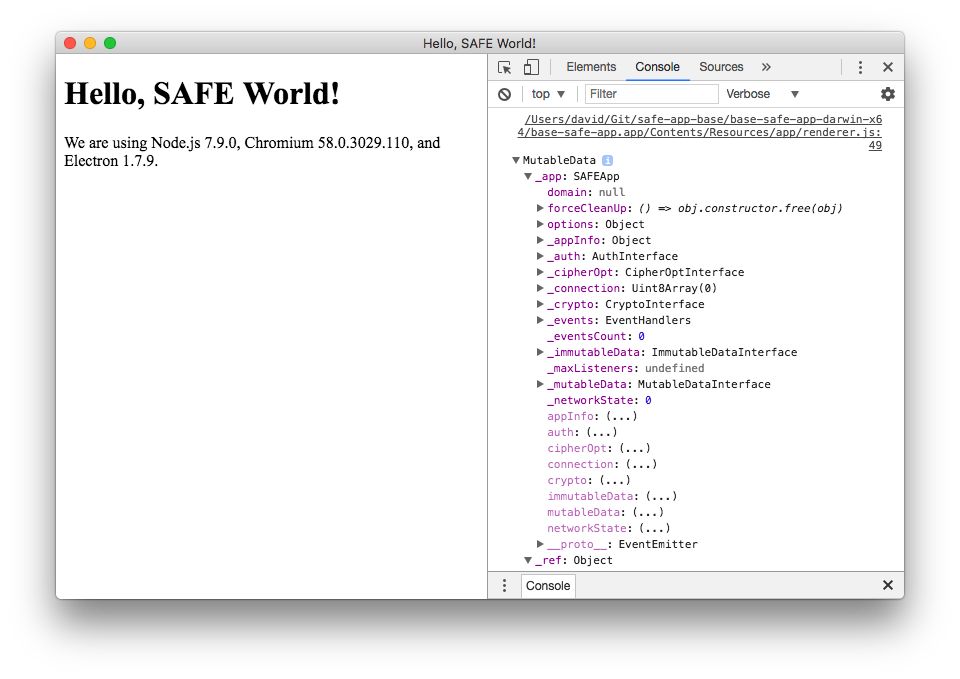
\includegraphics[width=\textwidth]{images/safe-app-base}
		\caption{SAFE App Base with newly created Mutable Data structure}
		\label{fig:safe-app-base}
	\end{center}
\end{figure}

It was a big setback for this project because if this simple example application didn't work then it would prove difficult to implement SAFE Wiki successfully. To help solve this a forum post\cite{safe-app-base-forummacfix} was created to discuss the issue with the community. The best approach would be to fix the example application before attempting the implementation in SAFE Wiki. After some conversation with numerous people I managed to deduce how to solve the problem, I made the fix myself myself\cite{safe-app-base-fix} and it got merged into the ``safe app base'' example application. The working ``safe app base'' can be seen in Figure \ref{fig:safe-app-base}. Problems with URI Schemes cropped up later on in development too, resulting in another forum post\cite{uri-scheme-ubuntu}. This time the issue was with support on Ubuntu. Thanks to the help of the creator of ``safe app base'' the issue was solved quickly.

\section{NFS Emulation}

To support the storage of ZIM files on the SAFE Network, SAFE Wiki makes use of the NFS emulation support that the \textit{Node.js API} has. This ``emulation'' is just a wrapper around Immutable and Mutable Data structures that makes working with ``files'' much easier. In SAFE Wiki nomenclature there is the concept of a \textit{ZIM folder}. This ``folder'' is really a Mutable Data structure that is emulated as a folder through NFS. Within this folder are placed the ZIM files that a given user uploads.

\subsection{ZIM Folder}

Every account on the SAFE Network has a number of Mutable Data structures by default that are called \textit{containers}. These \textit{containers} are similar to a ``home folder'' on a traditional OS in that they give applications structure (guidance) on where to store things. Such containers include: \_public, \_downloads, \_music, \_pictures, \_videos, etc. The ZIM folder that SAFE Wiki uses is stored within the \_public container because data stored within there can be ``un-encrypted'' or '`public'' data. Within the \_public container is placed a key value pairing where the key is ``zim'' and the value is the XOR Address of a Mutable Data structure that is the ZIM folder. When a user creates a ZIM folder they must specify a name. That name is then hashed to give a unique 256-Bit XOR address which is where the Zim folder is then stored. Thus through the name of the ZIM folder another user can locate the ZIM files uploaded by any other user.

\subsection{ZIM Files}

Once a user has created a ZIM folder they are then able to upload ZIM files to the network. This is achieved through the use of the NFS emulation support of the \textit{Node.js API}.  When a user uploads their ZIM file they give it a name, this name is important. This name is the ``file name'' of the file, meaning that within a given ZIM folder the ZIM file is stored against the name the user specifies.

\begin{figure}[h]
	\begin{center}
		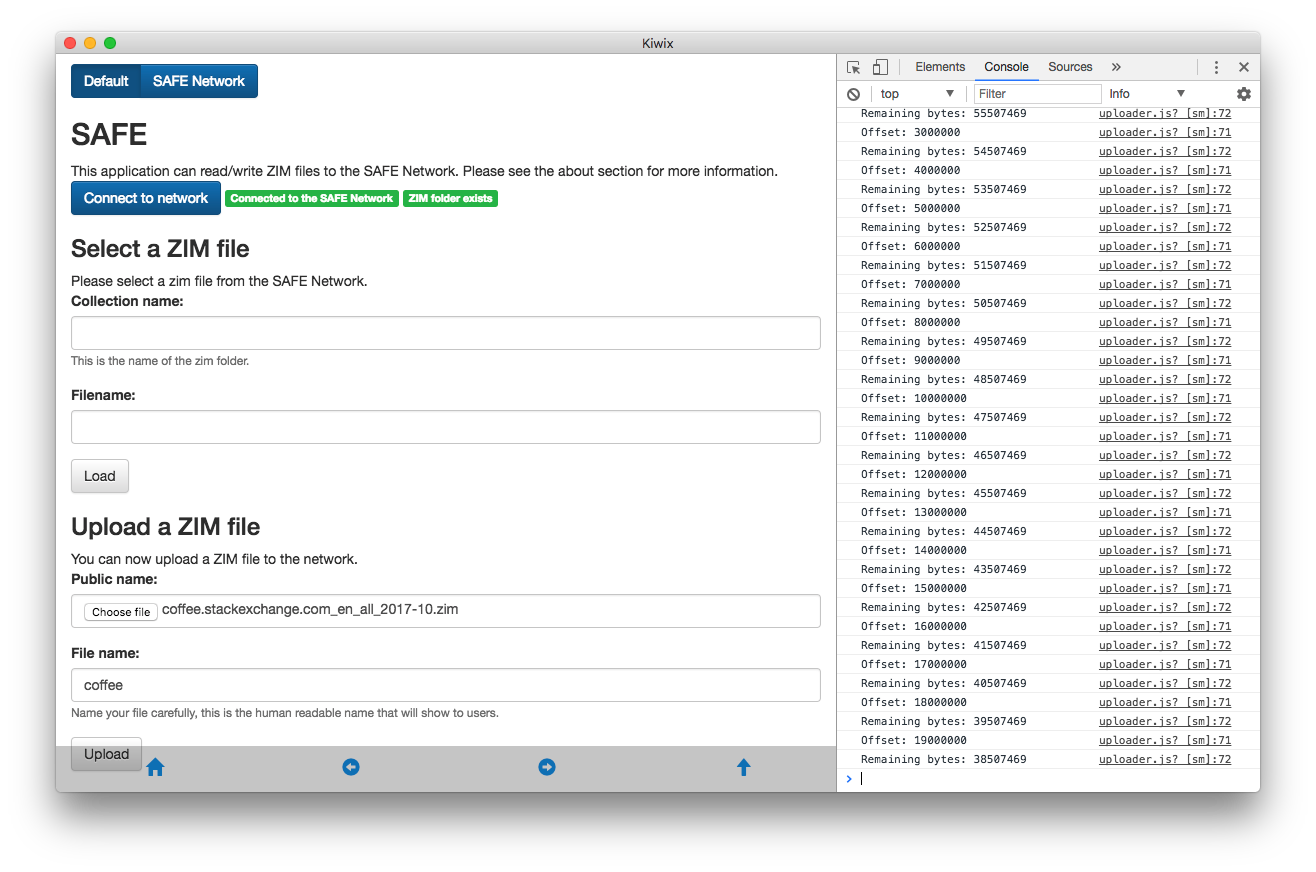
\includegraphics[width=\textwidth]{images/safe-wiki-uploading-coffee}
		\caption{Uploading the Coffee StackOverflow ZIM file to the SAFE Network}
		\label{fig:safe-upload-coffee}
	\end{center}
\end{figure}

To access a ZIM file, all a user has to provide SAFE Wiki with is the name of the ZIM folder and the name of the ZIM file within that folder. This approach means it is easy to share access to ZIM files, as names can be human readable they are as easy to share as website URLs. The resolution of the 256-Bit XOR address of the ZIM Folder is through hashing. As the ZIM folder was stored at the address corresponding to the name specified by the ``owner'', the address is then derivable by anyone else that knows that name. The way this is envisioned to be used is the name of the ZIM folder can correspond to the originator of the content then the filenames follow on logically from that. For example, ``Wikimedia'' could be the name of the ZIM folder then ``Wikipedia'' could be the name of the ZIM file. Meaning a user has two words to type in to browse the latest version of Wikipedia. As things are organised like this it then becomes logical to derive the location of other ZIM files. A user can deduce that to get to ``WikiVoyage'' is as simple as ``Wikimedia'' and ``WikiVoyage'`.

\section{Reading ZIM Files}
 
An important feature that is facilitated through the use of \textit{Data Maps}(Section \ref{subsec:self-encryption-data-map}) is being able to randomly seek through files. The \textit{Data Map} contains enough information about a file that arbitrary bytes can be read without having to download all data chunks. For ZIM files this is important, it is illogical for SAFE Wiki to have to download the entire Wikipedia so a user can browse a single article.

\begin{figure}[h]
	\begin{center}
		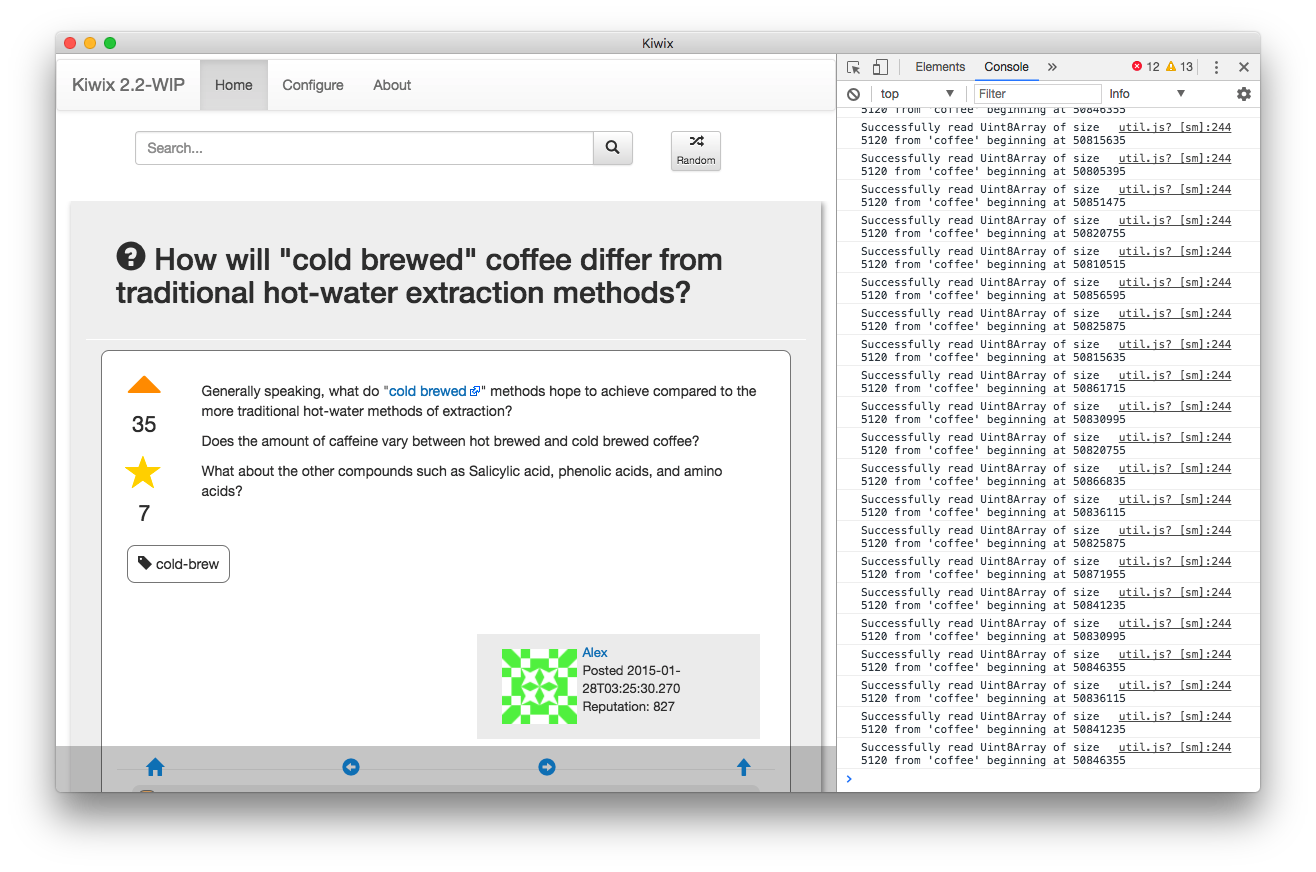
\includegraphics[width=\textwidth]{images/safe-wiki-browsing-coffee}
		\caption{Browsing a page from the StackOverflow Coffee ZIM file on the SAFE Network}
		\label{fig:browsing-coffee}
	\end{center}
\end{figure}

Kiwix JS by itself is setup to read ZIM files from local storage. To facilitate reading ZIM files from the SAFE Network, instead of reading a number of bytes (specified by ``begin'' and ``size'' in Figure\ref{fig:zim-read-code}) from local storage, the request is directed to the SAFE Network. Doing it this way is convenient because it doesn't require a complete overhaul of file reading within Kiwix JS. This approach, being more modular in design, means that the original functionality of Kiwix JS is maintained. You can select whether to read files locally or to read them from the SAFE network. The code to perform reading is shown in Figure \ref{fig:zim-read-code}. The \textit{zimFolder} that is a Mutable Data structure is emulated using NFS and the \textit{file} is fetched through the \textit{filename} specified by the user. To then read the required bytes is simple. In Figure \ref{fig:browsing-coffee} the console shows the reads from the network. The API and libraries handle all of the complexities of \textit{Data Maps} for you so reading from the network in this fashion is not complex once all the pieces are in place.

\begin{figure}[h]
\begin{lstlisting}[frame=single]
readZim (zimFolder, filename, begin, size) {
  return new Promise(async (resolve, reject) => {
    try {
      const nfs = zimFolder.emulateAs('NFS')
      let file = await nfs.fetch(filename)
      file = await nfs.open(file, CONSTANTS.FILE_OPEN_MODE.OPEN_MODE_READ)
      let data = await file.read(begin, size)
      file.close()
      resolve(data)
    } catch (error) {
      reject(error)
    }
  })
}
\end{lstlisting}
\caption{Code to read a ZIM file from the SAFE Network}
\label{fig:zim-read-code}
\end{figure}










